\chapter{\label{c:esd-concept}Demonstration of a plate capacitor electrostatic actuator with reduced seismic coupling}

\begin{itemize}
  \item Introduce Holger's paper~\cite{Wittel2015} \etal{}, discuss need for high voltages
  \item Actuators usually couple noise, which is why magnets are usually on a stage above the test masses. This necessarily limits range, as any actuation performed by the magnets will be filtered by 1/f
  \item Immunity to seismic noise due to turning points on graph from Holger's paper (see C.G. talk)
  \item HV power supply design considerations (bleed resistor, voltage requirements, etc.)
  \item HV power supply current limiting circuit explanation (called ``foldback limiting'', see Horowitz and Hill p694)
  \item HV power supply heatsink considerations: power produced by MOSFETs at maximum current rating (100 mA, produces 25 W of heat - see datasheets) - chose heatsinks to dissipate this heat and make installation of the board easy (can screw TO-220 casing to L-shaped brackets)
  \item HV amplifier design: pressure and temperature cut-offs (explanation of how it works), input/output signals, choice of connectors, routing of signals for ease of assembly (front panel disconnect, etc.)
  \item Protective earthing (how the removal of the ground supply from the GEO supply will clamp ground to Earth beyond 18 V)
  \item HV amplifier transfer function, usign both HV output (via voltage divider) and monitor output
  \item HV amplifier monitor noise measurement
  \item This experiment will inform the main SSM experiment.
  \item 10 ohm resistor on output of amplifier design to damp resonant RCL modes: resistor adds loss, so lowers the Q associated with any suspension or cable pickups
  \item ESDs are useful in particular for this expeirment because the mirror masses are small. Previously considered for GEO but the mirrors are too heavy for it to be effective.
  \item Immune to EM pickup, possibly, because there are no mirrors on the bottom stages of any suspension.

  \item Discuss how Andreas' design (with my modifications) was a first prototype, and we decided to redesign it afterwards because of various problems: requirement for a 5V offset at all times, the heat production (due to quiescent current) of the PA98s, lack of switchable whitening. New design incorporates this stuff, along with significant digital signalling thought, and quad channels. New connector to the vacuum feedthrough, too.
  \item Discuss digital signalling design: avoiding ground loops, the DB25-37 converter board, pull-up resistors, etc. Mention that we considered EtherCAT for this but decided it was too expensive (needs a dedicated block inside the amplifier box)
\end{itemize}

As described in Chapter\,\ref{c:speedmeter-control}, the \gls{ESD} is best employed as a high frequency actuator...

\section{Anticipated control loop}

\begin{figure}
  \centering
  \includegraphics[width=\columnwidth]{graphics/generated/from-svg/60-esd-experiment-control-loop.pdf}
  \caption[Control loop for the electrostatic drive experiment]{\label{fig:esd-ansys}ESD experiment control loop.}
\end{figure}

\section{Actuator requirements}

% ESD force gradient, from esd-ansys.pdf figure
\newcommand{\ESDFORCEGRAD}{\SI{-3.68}{\nano\newton\per\volt}}

% ESD maximum voltage
\newcommand{\ESDMAXVOLTAGE}{\SI{750}{\volt}}

% ESD maximum force, read from esd-ansys.pdf figure (gradient * voltage doesn't work because there's a non-zero y-intercept)
\newcommand{\ESDMAXFORCE}{\SI{-1.48e-6}{\micro\newton}}

There are a number of requirements for the power supply for the actuator electronics. Due to the nature of the actuator load--a capacitor formed from parallel plates--the power supply does not need to drive a significant current. On the other hand, the power supply will be modulated by the amplifier and sent to the plates, and the plates produce a field that will actuate directly upon the test masses, and so any noise present upon the power supply output can potentially limit the sensitivity of the experiment. In order to achieve significant actuation, it is also necessary to provide a high voltage supply to the amplifier. Simulations conducted with the finite element modelling package \emph{ANSYS} have found that, for a mirror geometry resembling that of the \SSMEXPT{}'s \glspl{ETM}, the force gradient will be \ESDFORCEGRAD{}, as shown in Figure\,\ref{fig:esd-ansys}. For a sufficient level of force actuation within the voltage isolation limit of our vacuum tank feedthroughs, a maximum feasible voltage across the capacitor appears to be in the region of \ESDMAXVOLTAGE{}, leading to a maximum mirror actuation force of \ESDMAXFORCE{}.
% ESD volts -> force from https://arran.physics.gla.ac.uk/wp/speedmeter/?p=4507

As this experiment is somewhat a technology demonstration for the main \SSMEXPT{}, it is worth keeping in mind its goals. For this reason, the actuator should provide suitably low output noise and sufficient channels for the purposes of the control of the full experiment. \note{Which means the displacement noise of the actuator should be less than xxx m/sqrt Hz}

\begin{figure}
  \centering
  \includegraphics[width=\columnwidth]{graphics/generated/from-python/60-esd-ansys.pdf}
  \caption[Simulations of the actuation force produced by the proposed electrostatic drive design]{\label{fig:esd-ansys}Simulations of the actuation force produced by the proposed \gls{ESD} design upon a \SI{100}{\gram} cylindrical test mass of diameter \SI{48.6}{\milli\meter} and depth \SI{24.5}{\milli\meter} resembling that of the \SSM experiment's ETMs. The plate separation and the position of the mirror with respect to the plates influence the level of force produced. \checkme{In practice it is most beneficial to have the mirror centre of mass aligned to the edge of the plates and the plates as close as possible to the mirror without touching.}}
\end{figure}

\subsection{Power supply}
To avoid the use of costly commercial power supplies, an attempt was made to build a \SI{\pm450}{\volt} supply using a mains transformer. This is documented in Appendix\,\ref{a:hv-power-supply}, though this design was not able to drive reactive loads due to design issues not realised until testing. As the amplifier contains capacitors that charge upon switch-on, this represented a reactive load that caused damage to the sensitive \glspl{MOSFET} present within the power supply. Instead, commercial Delta Elektronika power supplies were acquired.

\subsection{Noise budget}
\note{The actuator must not add more noise than we already expect from seismic etc...}

\section{\label{sec:hv-amplifier}High voltage amplifier}

A means of controlling the \gls{AC} component of the high voltage (\gls{HV}) supply is necessary to perform frequency-dependent corrections upon the mirror. Although the \gls{ESD}, and indeed the \SSM{} experiment, primarily require corrections at lower frequencies where seismic noise is dominant, it is beneficial to utilise an amplifier which can provide actuation up to many tens, if not hundreds, of \SI{}{\kilo\hertz}. This facilitates a transfer function which is flat across the vast majority of each experiment's measurement band, avoiding the roll-off at high frequencies due to the integrated circuits utilised within the high voltage amplifier. A flat transfer function makes the calibration of the actuator plant as part of the overall experiment as simple as possible. Another benefit of having a high bandwidth amplifier is the possibility to use it for common mode control loops, where laser frequency stabilisation can be split between feedback to the laser's piezoelectric transducer and actuators on the test masses.

The key component of a high bandwidth amplifier is the power op-amp. This class of op-amps typically utilises a \gls{MOSFET} design, and can provide high voltage output given a low voltage input. As an example, the Apex PA95 op-amps used in Advanced LIGO's \glspl{ESD} provide up to \SI{900}{\volt} output up to a frequency of around \SI{15}{\kilo\hertz}, and up to \SI{50}{\volt} at \SI{250}{\kilo\hertz}. The PA98 op-amp, also from Apex, provides an output of \SI{450}{\volt} nominally up to \SI{60}{\kilo\hertz}, potentially up to \SI{500}{\kilo\hertz} for a low capacitive load. For the purposes of this experiment, the choice was made to use the PA98 op-amp to provide the ability to study the effect of the actuator across a very wide bandwidth. To this end, an amplifier circuit utilising the PA98 was built based on a design used for the \AEIPROTOTYPE{}. This design provides up to \SI{\pm350}{\volt} output, and originates from a single-ended, \SI{350}{\volt} amplifier design where the PA98 is especially suited. Two notable modifications have been made, with a view to safety.

% claim about voltage output of PA95 comes from figure ``Power Response'' on p3 of PA95 datasheet (https://www.apexanalog.com/resources/products/pa95u.pdf)
% claim about voltage output of PA98 comes from figure 8: ``power Response'' on p7 of PA98 datasheet (https://www.apexanalog.com/resources/products/pa98u.pdf)

The first modification is the use of alternative high voltage connectors. The \AEIPROTOTYPE{} design called for two \emph{SHV} connectors carrying the separate +\gls{HV} and -\gls{HV} rails to the vacuum feedthrough on separate cables, with the vacuum system acting as the virtual ground between the two rails. While both cables are connected, this system is safe; however, if one cable is disconnected, a fault with the amplifier circuit can cause the vacuum system to become live. To avoid the possibility of this situation occurring in the \SSM{}, a Bulgin-type connector was used to combine the +\gls{HV} and -\gls{HV} rails in a single connector and cable. With this style of connector it is not possible to disconnect from the vacuum system any single \gls{HV} rail while leaving the other connected.

The second modification made to the amplifier circuit was the addition of a safety interlock mechanism. The breakdown voltage of the plate capacitors as a function of pressure, given by Paschen's Law, has a minimum in the region of \SI{e3}{} to \SI{e7}{\milli\bar} depending on the separation and geometry of the anode and cathode. In addition, related effects such as surface tracking can lead to arcing at voltages above \SI{50}{\volt} in low vacuum. Although the use of high voltage plate capacitors is in general safe at both atmospheric pressure and high vacuum (below \SI{e-6}{\milli\bar}), the act of pumping gas out of the vacuum system necessarily passes through pressures at which arcing can occur, so a safety mechanism was necessary.

\begin{figure}
  \centering
  \includegraphics[width=\columnwidth]{graphics/generated/from-python/60-esd-paschen.pdf}
  \caption[Minimum breakdown voltage between the two plates of the electrostatic drive for different separations]{\label{fig:esd-paschen}The minimum breakdown voltage between the two plates of the \gls{ESD} for different separations. This is calculated using Paschen's Law, assuming nitrogen gas and a flat plate geometry. The effect is a lot more complicated for real systems, where different plate geometries will have different relationships, but the steep slope at lower pressures shown here indicates that the apparatus used in the \gls{ESD} experiment will very likely avoid any problems with arcing as long as a suitable pressure-based interlock is utilised in the design of the electronics.}
\end{figure}

To prevent the possibility of arcing, a cut-off function was added to the circuit to prevent high voltage output unless a voltage above \SI{5}{\volt} is applied across terminals on the enclosure (see Figure\,\ref{fig:amplifier-interlock}). This threshold was chosen based on the monitor output voltage provided by a pressure gauge attached to the vacuum system. The monitor output varies logarithmically from \SI{0}{} to \SI{10}{\volt} for pressures between standard atmosphere and ultra-high vacuum. A voltage above \SI{5}{\volt} indicates a pressure below \SI{e-5}{\milli\bar}.

% pressure vs voltage claim from speedmeter labbook, at https://arran.physics.gla.ac.uk/wp/speedmeter/2015/01/30/esd-hv-amplifier-pressure-cutoff/

\begin{figure}
  \centering
  \includegraphics[width=\columnwidth]{graphics/generated/from-svg/60-amplifier-interlock.pdf}
  \caption[High voltage amplifier pressure interlock circuit]{\label{fig:amplifier-interlock}HV amplifier pressure interlock circuit. An op-amp (N8A) compares the voltage from a fixed \SI{5}{\volt} reference against an externally supplied voltage (``in'') intended to be connected to a pressure gauge. When the external voltage is lower than \SI{5}{\volt} (indicating suitably high vacuum), the op-amp's output is negative and transistor T14 is not open. In this scenario the current from the +\SI{15}{\volt} supply can flow through optoisolators N7, N9, N12 and N13 to provide the supply rails for the PA98s. When the external voltage is higher than \SI{5}{\volt} (indicating a pressure above the safe limit), the op-amp's output is positive. As the op-amp's output is fed back to the \emph{positive} input, the op-amp quickly reaches its positive supply rail, \SI{15}{\volt}. This operates T14 which opens a low-resistance path to ground for the current that would otherwise operate the optoisolators, effectively turning off the PA98s' supply rails.}
\end{figure}

\subsection{\label{sec:signal-and-noise-paths}Signal and noise paths}
The \gls{HV} amplifier is designed to have a very wide bandwidth, and the power amplifier has been chosen with this goal in mind. The amplifier circuit, however, contains more than just the power amplifier, but also filtering and safety mechanisms in the form of additional integrated circuits and other passive and active components. The control input from \gls{CDS} is a differential signal, and any common mode noise that may have entered in each channel on the way to the amplifier is to a great extent removed by a balanced line receiver present at the amplifier's input. This outputs a single-ended signal which is split into two parts, with one being inverted via a buffer op-amp, and these two signals are sent to their respective power amplifiers. Additional op-amps also control the supply voltage provided to each power amplifier. To prevent high current in-rush when the power supply is attached to the amplifier--as reactive components such as capacitors and inductors accumulate charge--an op-amp limits the current to a level low enough for the power supply to provide without locking.

In \gls{CDS}, the signal $S$ is sent from the digital to the analogue domain via \glspl{ADC}, where it is split into two channels, $A$ and $B$, containing the same signal but with opposite sign. These signals are sent to the amplifier in a two-core cable. As laboratories inevitably contain stray electromagnetic fields, channels $A$ and $B$ pick up noise $n_{A}$ and $n_{B}$, respectively:
\begin{align}
  A &= S + n_{A}, \\
  B &= -S + n_{B}.
\end{align}
These noise sources can be further represented in terms of common and differential modes at the amplifier input, $n_{\left(+\right)}$ and $n_{\left(-\right)}$, respectively:
\begin{align}
  n_{\left(+\right)} &= n_{A} + n_{B}, \\
  n_{\left(-\right)} &= n_{A} - n_{B}.
\end{align}
The purpose of this so-called \emph{differential sending} is to allow $n_{\left(+\right)}$ to be cancelled at the amplifier. Injecting channels $A$ and $B$ into an op-amp with high \emph{common-mode rejection}, we get:
\begin{align}
  S_{\text{out}} &= G_{\left(-\right)} \left(A - B\right) + G_{\left(+\right)} \frac{\left(A + B\right)}{2} \\
                 &= G_{\left(-\right)} \left(2S + n_{\left(-\right)}\right) + G_{\left(+\right)} \frac{n_{\left(+\right)}}{2},
\end{align}
where $G_{\left(-\right)}$ and $G_{\left(+\right)}$ are the op-amp's differential and common mode (power) gains, respectively.

As the original signal produced by \gls{CDS} is inverted in one channel, each channel contains purely differential signal, but the noise picked up by each channel is in both the differential and common modes. An op-amp's ability to remove common mode noise between its inputs is typically expressed as its \emph{common mode rejection ratio} (\gls{CMRR}), defined as the logarithm of the ratio of the differential and common mode gains:
\begin{equation}
  \text{CMRR} = 20 \log_{10} \left( \frac{G_{\left(-\right)}}{G_{\left(+\right)}} \right),
\end{equation}
with the resulting number expressed in decibels. Within the amplifier, the signals are subtracted by an AD829 with $\text{CMRR} = 120$ (at \SI{1}{\kilo\hertz}) configured with $G_{\left(-\right)} = 1$, resulting in only $5 \times 10^{-7} n_{\left(+\right)}$ making its way to the output (neglecting imbalances in nearby components such as resistors), making it comparible or less significant than the output noise of the op-amp itself. As the channels are physically close to one another as they are sent to the amplifier--contained within the same shielded cable--most noise pickup is common to both channels and so $n_{\left(-\right)}$ tends to be small for frequencies below a few \SI{}{\giga\hertz}. Using a receiving op-amp with sufficiently high \gls{CMRR}, a desired control signal can be sent from \gls{CDS} to the amplifier without the addition of significant noise.

% small differential noise claim: f = c/lambda, assume lambda has to be less than the channel separation in a cable, roughly 1mm, so 3e8 / 1e-3 = 3e11 = 300 GHz.

The gain of the amplifier can be determined from inspection of the path an input signal takes to the output... \note{discuss how gain arises in circuit}

\section{\label{sec:hv-psu-amp-measurements}Measurements with power supply and amplifier}

With the power supply connected to the amplifier, the power supply was observed not to work. On closer inspection it was revealed that the \glspl{MOSFET} used to regulate the output voltage were failing irreversibly immediately after switch-on. As this effect was not observed for constant load (see Section\,\ref{sec:hv-psu-tests}), it is thought that it was due to a combination of two characteristics of the system. The amplifier's current draw is initially larger on the positive rail than on the negative rail \checkme{is this the correct way round?}. The presence of inductors (in the form of the mains transformer and the \gls{AC} filtering chokes in both the power supply and amplifier), which due to tolerances can have slightly imbalanced filtering, can lead to the creation of parasitic reverse voltages exceeding each \gls{MOSFET}'s rating. Subsequent examination of power supply designs for amplifier electronics in the literature reveals that it is common practice to build protective circuitry alongside many of the components of the general power supply design shown in Figure\,\ref{fig:hv-power-supply}, to prevent such issues with reactive loads (see, for example, Figure\,9.110 of \cite{Horowitz2015}). As it was impractical to retrofit such protective circuitry into the power supply as designed, the decision was taken to instead purchase commercial \emph{Delta Elektronika ES 150} power supplies for use with the amplifier. The power supply, as designed, may prove more useful to future experiments involving loads with lower reactance.

\subsection{Amplifier transfer functions}
\note{Describe measurement: use of voltage divider, need to take into account impedance of the send box in its design, bandwidth of each measurement: CDS up to 10 kHz, SR785 up to 100 kHz, Agilent up to MHz. Describe monitor and \gls{HV} rail outputs, and how we avoid ground loops (isolated case from double LEMO and monitor outputs.}

The presence of stray capacitance at the inputs and outputs of these additional integrated circuits can have an influence upon the overall response of the amplifier as a function of frequency. It is beneficial, therefore, to check that the frequency response of the amplifier is dominated by the power amplifier and not by some auxiliary component.

\subsection{Noise measurements}

\note{Spectral density noise with SR785}

\section{\label{sec:hv-amplifier-alt}Further amplifier design iteration}
\note{Discuss new design: why it was felt necessary, what we fixed/changed, how it performs, etc...}

\note{Discuss safety features: new interlock that requires a digital LOW signal, which is pulled low by CDS. Same temperature cut-offs as before. 45k resistors on output to limit current to non-lethal levels. Warning label on box. Protective earth.}

\note{45k resistor gives 27 nV/sqrt(Hz) noise - is this significant?}

\note{Plot of noise budget for amplifier: PA95 input and output noise, Johnson noise, requirement in terms of displacement?}

\note{Short note on enclosure: 19 inch rack enclosure, front panel with LEDs, on button, etc.}

\begin{figure}
  \centering
  \includegraphics[width=\columnwidth]{graphics/generated/from-svg/60-hv-amplifier-signal-path.pdf}
  \caption[High voltage amplifier signal schematic]{\label{fig:hv-amp-signal-path}Signal path. \note{Differential receiving, switchable 10dB dewhiteners, test points, clamp diodes, amplifier with appropriate power resistors, voltage divider for monitor}}
\end{figure}

\begin{figure}
  \centering
  \includegraphics[width=\columnwidth]{graphics/generated/from-svg/60-hv-amplifier-soft-start.pdf}
  \caption[High voltage amplifier soft-start schematic]{\label{fig:hv-amp-soft-start}Soft-start. \note{Mostly from Andreas' design. Optoisolators, optocouplers, choke, 1.5KE voltage clamp, charger circuit.}}
\end{figure}

\begin{figure}
  \centering
  \includegraphics[width=\columnwidth]{graphics/generated/from-svg/60-hv-amplifier-interlock.pdf}
  \caption[High voltage amplifier interlock schematic]{\label{fig:hv-amp-interlock}Interlock. Four temperature sensors in TO-220 packages for easy attachment to metal. Positive feedback trip switch. CMOS switches (interlock one pulled to 15V). Bypass jumpers. AND gate. 1M resistor to clamp voltage to a ground reference.}
\end{figure}

\begin{figure}
  \centering
  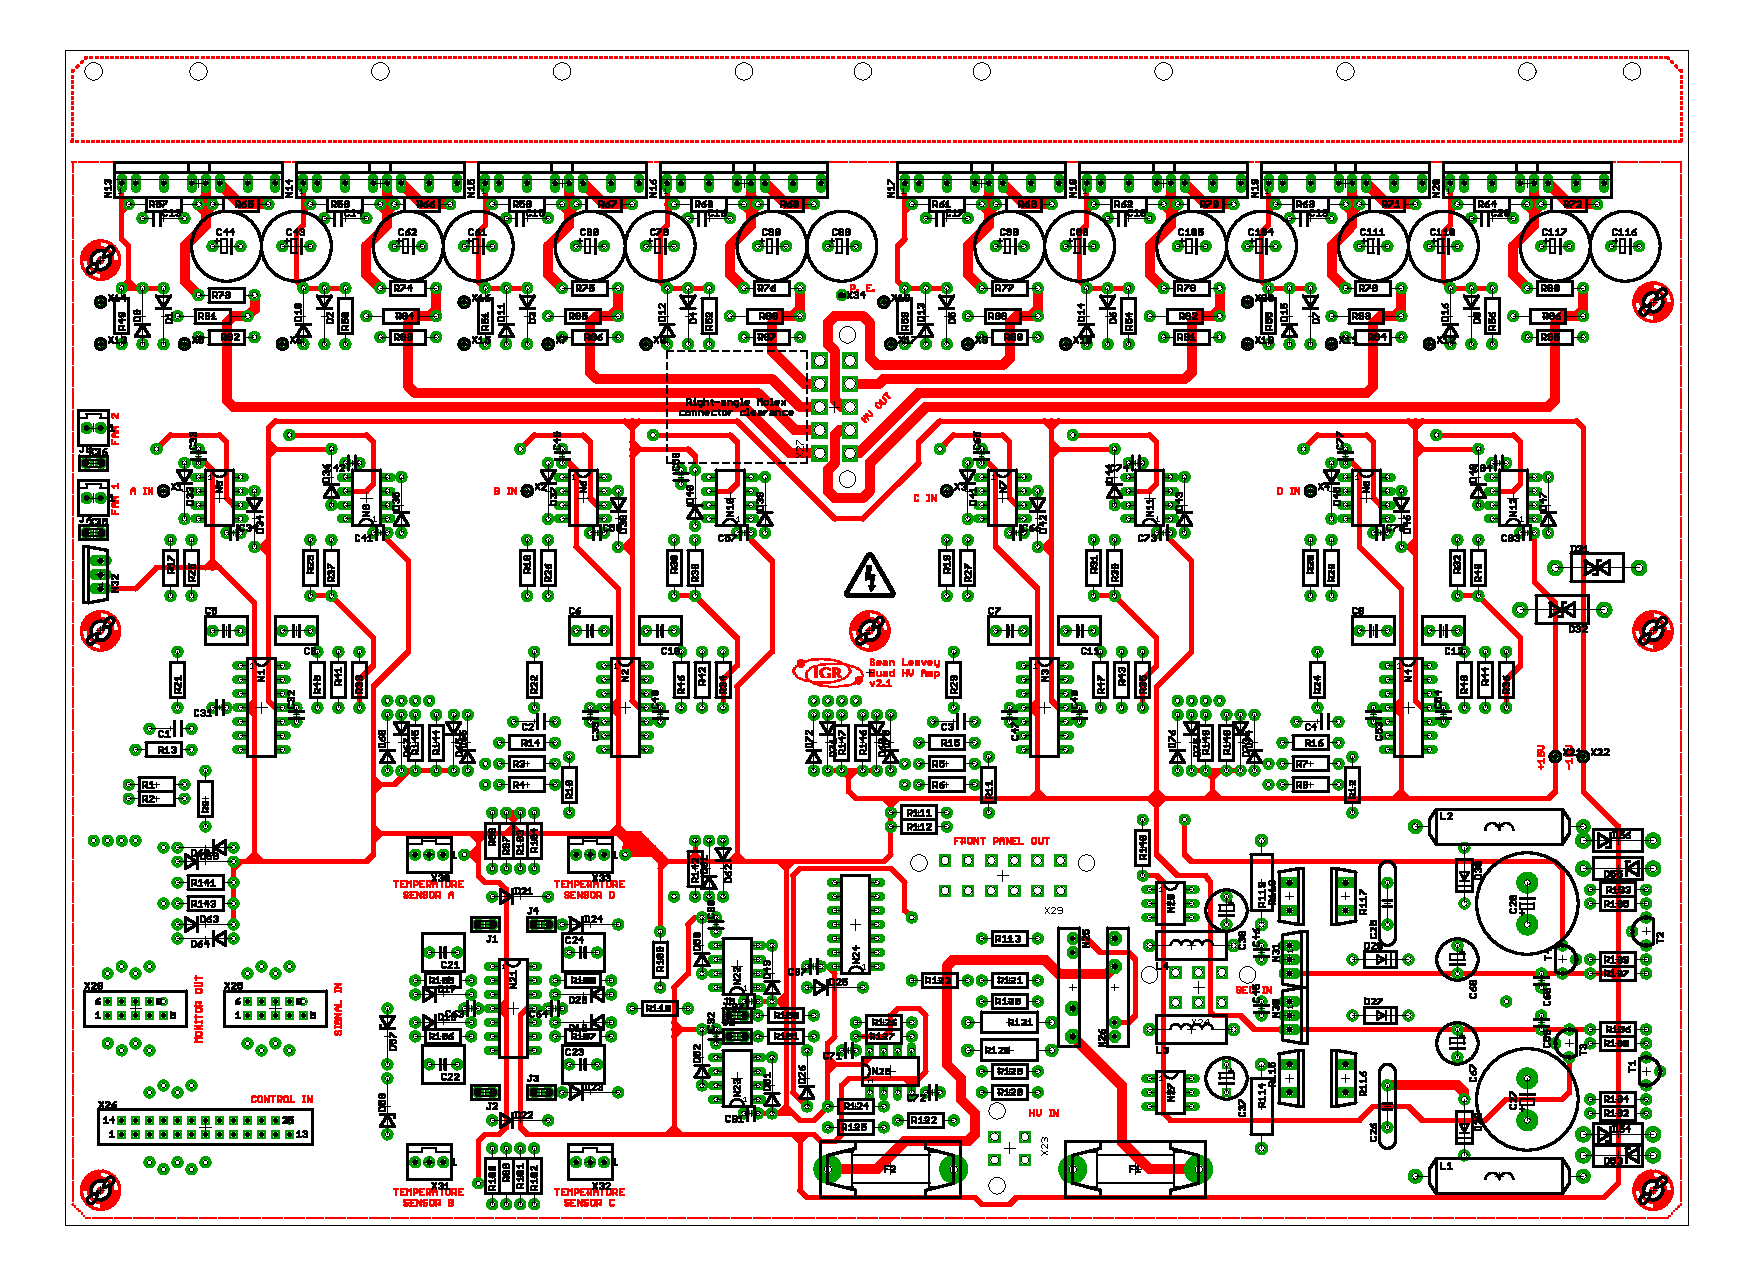
\includegraphics[width=\columnwidth]{graphics/60-hv-amp-top.pdf}
  \caption[High voltage amplifier board layout (top)]{\label{fig:hv-amp-top}Top view of the high voltage amplifier printed circuit board. In the lower left corner there are IDC connectors for the signal and control inputs and the monitor outputs. These connect via ribbon cables to the inside of the amplifier enclosure's front panel. Various other sockets are present in the lower half and upper centre of the board for high and low voltage inputs and outputs. The eight PA95 amplifier ICs are situated near the top of the board, and some space is left at the top of the board to allow these amplifiers to be attached to heat sinks. The copper layer immediately below the heat sink locations is isolated from the board's main ground plane to prevent the heat sinks from shorting the board's ground to earth. The bottom view is shown in Figure\,\ref{fig:hv-amp-bottom}.}
\end{figure}

\begin{figure}
  \centering
  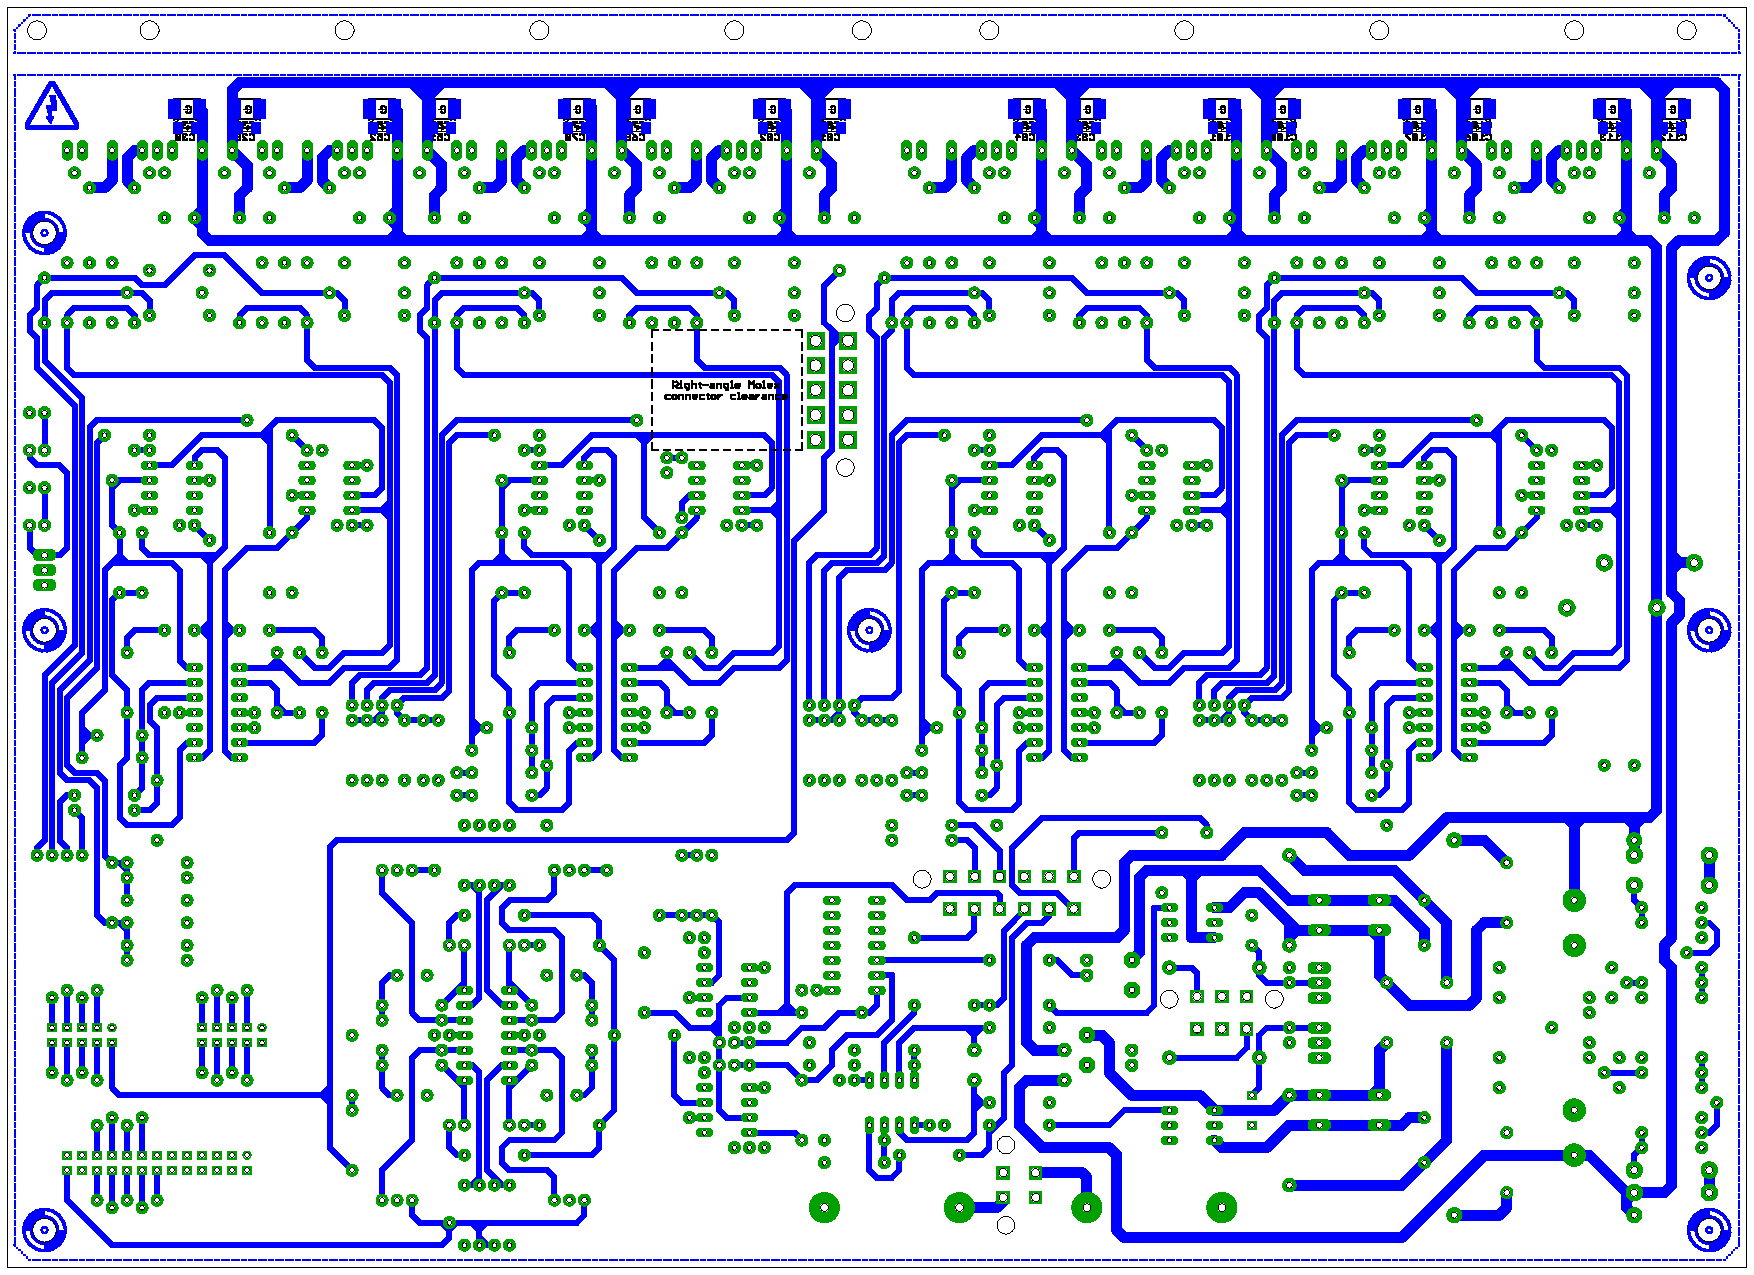
\includegraphics[width=\columnwidth]{graphics/60-hv-amp-bottom.pdf}
  \caption[High voltage amplifier board layout (bottom)]{\label{fig:hv-amp-bottom}Bottom view of the high voltage amplifier printed circuit board. The lower right corner of the board contains the ``soft start'' circuitry to charge the high voltage capacitors on the board, and the high voltage supply rails are routed from here to the top of the board where they are fed to each of the eight PA95 ICs. The remaining tracks on the bottom are predominantly used for board signal routing. The top view is shown in Figure\,\ref{fig:hv-amp-top}.}
\end{figure}

\begin{figure}
  \centering
  \includegraphics[width=\columnwidth]{graphics/generated/from-python/60-new-amplifier-dewhitening-sims.pdf}
  \caption[Simulated dewhitening filter frequency response]{Dewhitening, simulated with LISO.}
  \label{fig:new-amplifier-dewhitening-sims}
\end{figure}

\begin{figure}
  \centering
  \includegraphics[width=\columnwidth]{graphics/generated/from-python/60-new-amplifier-dewhitened-tfs.pdf}
  \caption[Frequency response of the high voltage amplifier's channels with dewhitening enabled]{Second amplifier transfer functions with dewhitening enabled. The expected performance of the dewhitening filter from theory is shown in \checkme{green} alongside the transfer functions of each channel. The curves agree closely, showing that the implemented filter operates as expected. The mismatch at high frequency is caused by the anti-aliasing filters implemented in CDS, which aggressively filter signals above \checkme{a few \SI{}{\kilo\hertz}} (\note{see Chapter 4 AA filter section}).}
  \label{fig:new-amplifier-dewhitened-tfs}
\end{figure}

\begin{figure}
  \centering
  \includegraphics[width=\columnwidth]{graphics/generated/from-python/60-new-amplifier-channel-one-tfs.pdf}
  \caption[]{}
  \label{fig:new-amplifier-dewhitened-tfs}
\end{figure}

\begin{figure}
  \centering
  \includegraphics[width=\columnwidth]{graphics/generated/from-python/60-new-amplifier-coherence.pdf}
  \caption[High voltage amplifier cross-channel coherence]{Second amplifier channel coherence.}
  \label{fig:new-amplifier-coherence}
\end{figure}

\section{Digital control signals}
\note{Describe digital signalling infrastructure: converter box, etc.}

\begin{figure}
  \centering
  \includegraphics[width=\columnwidth]{graphics/generated/from-svg/60-db25-cable.pdf}
  \caption[DB25 cable assembly]{DB25 cable assembly for routing of digital signals. As this cable provides access to the GEO voltage and current supply, it was chosen to be a unique connector in the experiment such that it cannot be accidentally attached to a device not intended for digital signalling.}
  \label{fig:db25-cable}
\end{figure}

\section{Wiring scheme}
\note{Discuss wiring diagram for ESD experiment...}

\section{Noise budget}
\note{Project electronic noise into displacement, show requirement. See seismic coupling from Stefan and Holger's SVN repo, input noise to electronics x40, etc...}

\section{Experiment}

\subsection{Transfer functions}
\note{Hopefully these are flat, just like the actuator TFs, once the cavity effect is removed...}

\section{Outlook}